\section{Oscillations}

\bi

\i Recall that a musical note typically has a characteristic 
pitch (fundamental frequency), so its associated pressure wave 
{\em repeats} over time.

\i Hence, understanding repeated motion 
is important for understanding both the production and 
perception of sound.

\ei

%%%%%%%%%%%%%%%%%%%%%%%%%%%%%%
\subsection{Periodic motion}

\bi

\i Oscillation: {\em any} motion that repeats itself.
Also called periodic motion.

\i Examples / demos: Mass on a spring, swinging pendulum,
a vibrating guitar string, a vibrating air column in a tube,
the Earth rotating around its axis, the Earth orbiting the Sun,
etc.

\i Period: time needed to complete one cycle ($T$)

\i Frequency: number of cycles completed in one second ($f$)

\i Relationship between period and frequency:
%
\be
f=\frac{1}{T}
\ee
%

\i Amplitude: 1/2 peak-to-peak displacement or extent of the motion
(usually denoted by $A$, sometimes $x_0$ or $\theta_0$)

\i Periodic motion is thus characterised by its fundamental frequency
$f=1/T$, its amplitude, and the shape of the wave as a function of
time (called the waveform).

\i In the context of sound, the fundamental frequency corresponds to
pitch, the amplitude to loudness or sound intensity, and the waveform 
to the timbre or tone quality of the sound.
%(Note: We will see later that the perceived loudness of a sound
%actually depends on the {\em square} of the amplitude.)

\i Different waveforms with the same fundamental frequency sound 
differently due to the presence of higher harmonics (more on this
later).

\i Examples of different waveforms:
sine, triangle, square wave, sawtooth, pulse, random noise, and
the sum of two sine waves with slightly different fundamental 
frequencies (hear beats for this last example).

\i \demo Use playsound.m routine to listen to these different sounds.

\i \exer The frequency range of human hearing is roughly 
20~Hz to 20~kHz.
This is a factor of $1000$ or roughly 10 octaves 
($2^{10} = 1024$) in frequency.

Calculate the associated periods.

\ans
%
\begin{align}
20~{\rm Hz}:
\quad\quad
&T = \frac{1}{20~{\rm Hz}} = 0.05~{\rm s} = 50~{\rm ms}
\\
20~{\rm kHz}:
\quad\quad
&T = \frac{1}{20~{\rm kHz}} = 5\times 10^{-5}~{\rm s} = 50~\mu{\rm s}
\end{align}
%

\i The pressure variation range of human hearing at
1000~Hz is 
roughly $2\times 10^{-5}~{\rm Pa}$ (threshold of hearing)
to $20~{\rm Pa}$ (threshold of pain).
This is a factor of $10^6$ in pressure variation or $10^{12}$
in intensity (${\rm Watt/m}^2$).
Compared to standard atmospheric pressure $P_{\rm atm} = 10^5~{\rm Pa}$,
these values are only $2\times 10^{-10}$ and 
$2\times 10^{-4}$ of atmospheric pressure, respectively.
So even at the threshold of pain, the pressure change is only a 
few parts in $10^4$ of atmospheric pressure!

\i In contrast, the frequency range for human vision is 
only a factor of 2 (so 1 octave); 
and the intensity range of human vision is only a factor of
$10^5$ (versus $10^{12}$ for human hearing).
{\em Thus, the human ear is a much more sensitive device than the 
human eye!}

\ei

%%%%%%%%%%%%%%%%%%%%%%%%
\subsection{Simple harmonic motion}
\bi

\i Simple harmonic motion (SHM) is periodic motion with
a sinusoidal dependence
%
\be
x(t) = 
A\,\sin(2\pi f [t-t_0]) = A\,\sin(2\pi f t-\theta_0)
\ee
%
Note that the term proportional to $t_0$ (or $\theta_0$) just
shifts the sine curve to the right by $t_0$.

\i Recall from trigonometry that the sine and cosine functions 
can be defined with respect to a point $P$ on the unit circle:
%
\be
y = \sin\theta\,,\qquad
x = \cos\theta
\ee
%
and repeat whenever $\theta$ changes by $360^\circ$ or 
$2\pi$ radians (Figure~\ref{f:sine-cosine}).
%
\begin{figure}[htbp]
\begin{center}
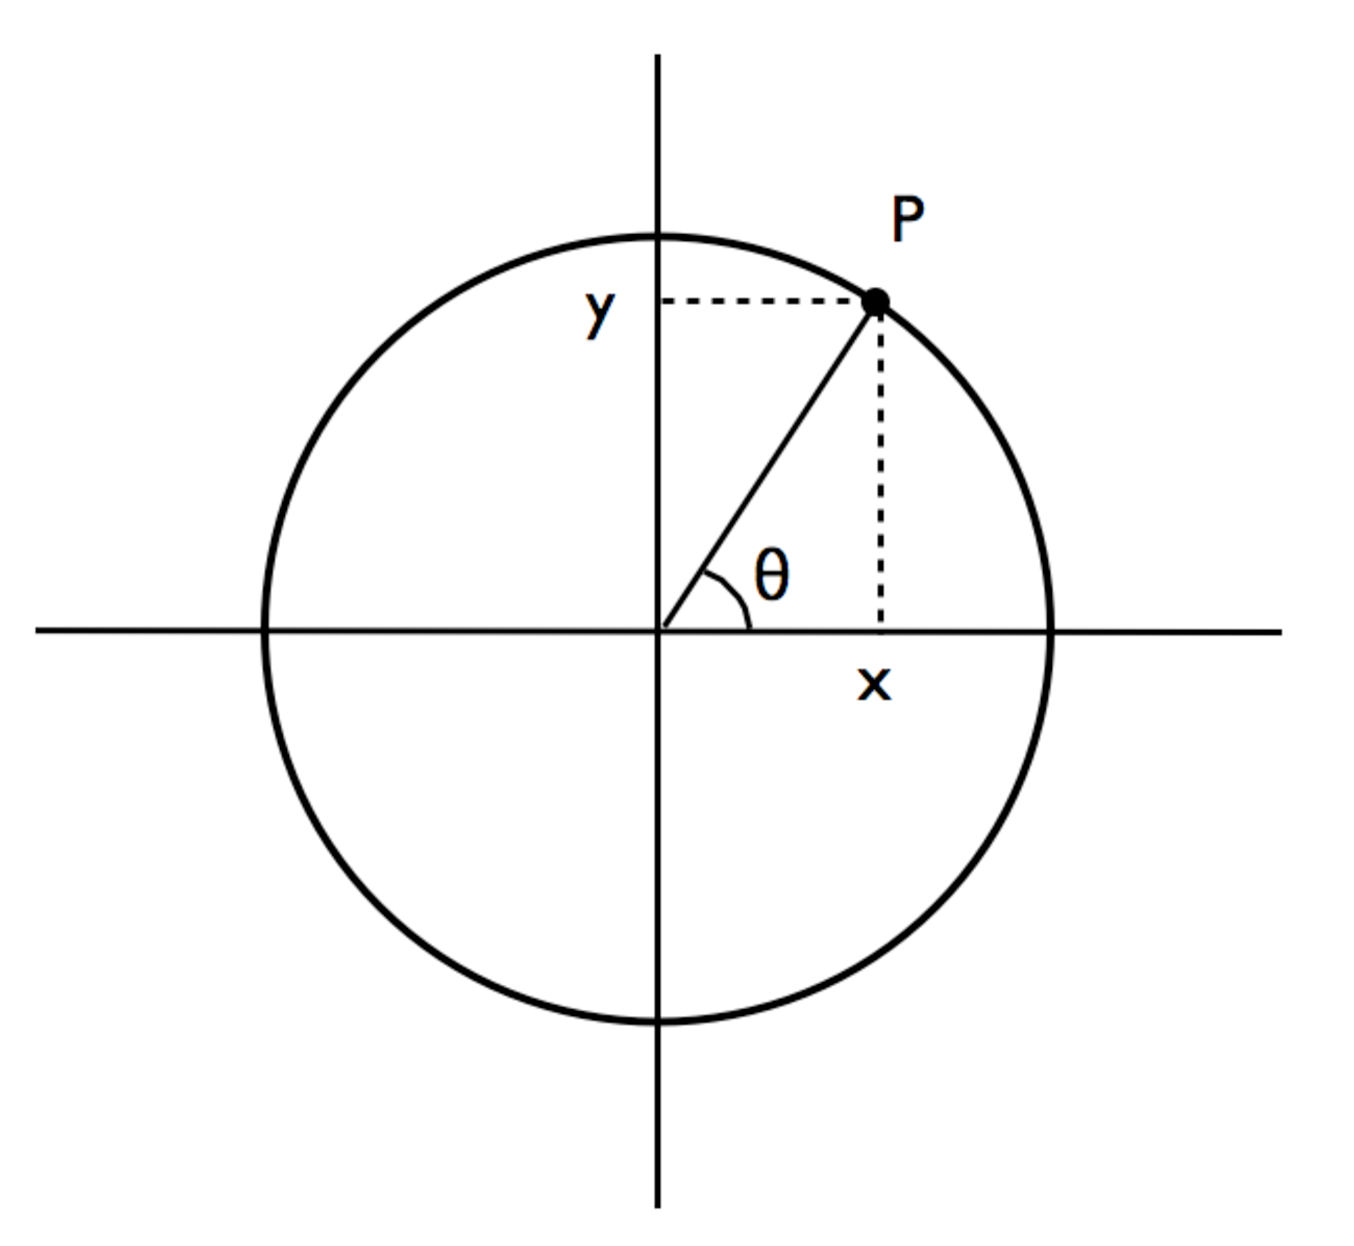
\includegraphics[width=.40\textwidth]{circle-theta}
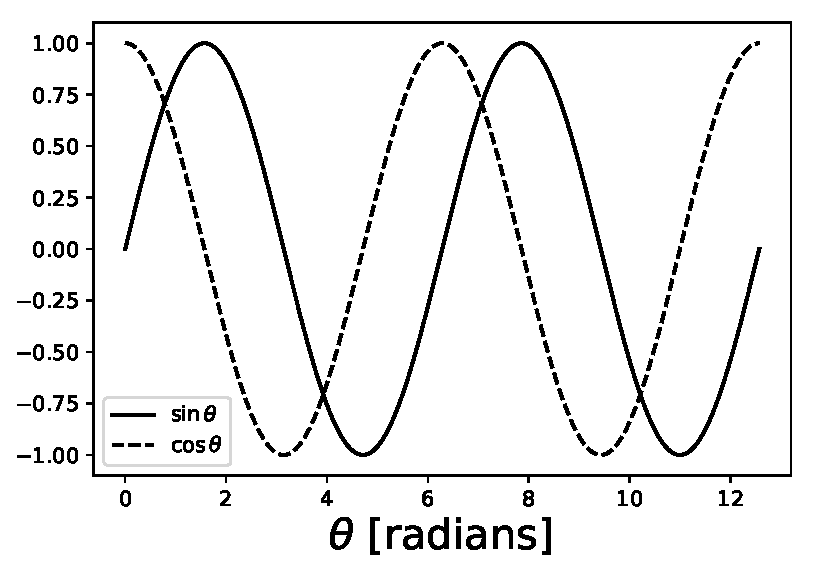
\includegraphics[width=.45\textwidth]{sine-cosine}
\caption{Left panel:
Point $P$ on a unit circle (radius equal to one)
making an angle $\theta$ with respect
to the $x$-axis.
Right panel: Plots of $\sin\theta$ and $\cos\theta$.}
\label{f:sine-cosine}
\end{center}
\end{figure}
%

\i Simple harmonic motion is produced whenever there is a
{\em linear restoring force} about a position of stable equilibrium.

Linear means that the force is directly proportional to the
displacement of an object away from its equilibrium position;
in other words, if you double the displacement you double the
force.

Restoring means that the force is always directed in such a 
way as to try to bring the object back to its equilibrium 
position.

\i One example of a linear restoring force is the force exerted 
by a stretched or compressed spring on a mass:
%
\be
F_{\rm spring} = -kx
\ee
%
where $k$ is the spring constant (which tells how stiff
the spring is) and $x$ is the diplacement of the mass $m$
away from the equilibrium position.
The minus indicates that the force is directed back toward
the equilibrium position.

\i The period and frequency of the associated SHM are
given by
%
\be
T = {2\pi}\sqrt{\frac{m}{k}}\,,
\quad
f = \frac{1}{2\pi}\sqrt{\frac{k}{m}}
\ee

\i Note that the period is independent of the amplitude
of the oscillation.
Also, larger masses have longer periods of 
oscillation, while stiffer springs have shorter periods.

\i \demo Illustrate the above by changing the amount of mass
attached to a spring.

\i Another example of a linear restoring force is the force 
(or more precisely the torque $\tau$) 
exerted by gravity on a swinging pendulum bob
%
\be
\tau =  -mgL\,\theta
\ee
%
where $L$ is the length of the pendulum,
$g$ is the acceleration due to gravity ($g\approx 10~{\rm m/s}^2$),
and $\theta$ is the angular displacement of the pendulum 
bob away from equilibium.

\i We are assuming here that the angular displacements
are small, i.e., $\theta \ll 1$.
If we allow large angular displacements, then the force becomes 
non-linear and the motion is no longer simple harmonic
(see below).

\i The period and frequency of the associated SHM are
given by
%
\be
T = {2\pi}\sqrt{\frac{L}{g}}\,,
\quad
f = \frac{1}{2\pi}\sqrt{\frac{g}{L}}
\ee

\i Note that the period is again independent of the amplitude
of the oscillation.
Also, longer pendula have longer periods of oscillation, and
the period is {\em independent} of the mass of the pendulum bob.

\i \demo Illustrate the above by changing the length of the 
pendulum, and then the mass of the pendulum bob.
(Parent and child swinging on separate playground swings
have the same period, despite their different masses.)

\i \demo
Use the program periodicmotion.m to illustrate the affect
of non-linear restoring forces on the waveforms of the 
resulting period motions.
Listen to the associated sounds and notice the presence of 
higher harmonics.

\ei

%%%%%%%%%%%%%%%%%%%%%%%%%%%%%%%%%%%%%%%%%%%%%%%%%%%%%%%
\subsection{Damped oscillations}

\bi

\i Real-world oscillations eventually damp out due to 
friction and air resistance.

\i A simple form of a damping (or drag) force has the form
%
\be
F_d = - b v
\ee
%
where $v$ is the velocity of the mass, and $b$ is some (positive) 
constant that specifies the strength of the damping.
An example of such a force is the drag force on a moving car 
due to air resistance.

\ei

%%%%%%%%%%%%%%%%%%%%%%%%%%%%%%%%%%%%%%%%%%%%%%%%%%%%%%%
\subsection{Driven oscillations}

\bi

\i In order to sustain an oscillation that has damping, it 
is necessary to supply energy from outside.
Such an outside force is called a {\em driving force}.

\i For damped, driven oscillations there are three 
forces acting:
%
\begin{align}
F_s&=-kx
\quad
({\rm restoring\ force})\\
F_d&=-bv
\quad
({\rm damping\ force})\\
F_{\rm driving}&=F_0\cos(2\pi f t)
\quad
({\rm driving\ force})
\end{align}
%
where $F_0$ is the amplitude of the driving force and 
$f$ is the driving frequency, which might be different 
from the natural frequency of the oscillation 
$f_0= (1/2\pi)\sqrt{k/m}$.

\i After an initial transient period corresponding to
the damped (undriven) motion, the motion of the
mass will be simple harmonic with a frequency equal to the driving 
frequency $f$.
The phase and amplitude of the motion will depend on the
relationship between the driving
frequency $f$ and the natural frequency $f_0$.

Assuming that the damping is small, 

(i) for $f\ll f_0$, the motion of the mass is 
in phase with the driving force, and has an amplitude equal 
to the driving force amplitude $F_0/k$.

(ii) for $f\gg f_0$, the motion of the mass is 
180$^\circ$ out of phase with the driving force, and
has an amplitude that tends to zero as the driving frequency
tends to infinity.

(iii) for $f\approx f_0$, the motion of the mass is
90$^\circ$ out of phase with the driving force,
and has an amplitude that can be much larger than the
driving force amplitude $F_0/k$. 

\i The case where $f\approx f_0$ is called {\em resonance}.

\i \demo Illustrate these three different cases using
a simple pendulum, moving the pivot point by hand with 
different frequencies.

\i \demo Illustrate these three different cases using
the program dampeddrivengui.m
(choose damping=0.05, amplitude=0.2, frequency=variable).

\i Other examples of resonance:

- pushing a child on a swing or pumping with your legs 

- car bump analogy: the size and spacing of bumps is 
most effective at slowing a car when they are chosen 
to be approximately the same size of the car's wheels 
and the spacing between the front and back wheels of
the car

- blowing over a Coke bottle to produce a note:
the bottle has natural frequencies appropriate for 
a tube closed at one end;
blowing is the driving force having 
contributions from all frequencies (basically noise);
only those frequencies of the blowing that match 
the natural frequency of the bottle are in resonance

- a vibrating guitar string doesn't 
produce much sound on its own, but it acts as the 
driving force on the body of the guitar, which is 
coupled to the string via the bridge.
If the body of the guitar has natural frequencies 
close to the frequency of the 
vibrating string, then the guitar body resonates 
and produces large amplitude oscillations which are 
easier to hear.

- a tuning fork mounted on a sound box is the
same as the guitar string example

- resonance between two pendula having the same 
length (coupling via the rocking support rod) 
or between two tuning forks having 
the same frequency (coupling via the air)

\ei

%%%%%%%%%%%%%%%%%%%%%%%%%%%%%%%%%%%%%%%%%%%%%%
\subsection{The not-so-simple simple pendulum}
\label{s:notsosimple}

\bi

\i If you allow large amplitude angular displacements,
the motion of a simple pendulum is no longer simple harmonic
since the restoring force is no longer linear.

\i The damped, driven simple pendulum with a
non-linear restoring force exhibits a variety of
possible motions ranging from simple harmonic, to
periodic, to chaotic.

\i Chaotic motion is non-periodic, unpredictable 
motion associated with deterministic equations.
The unpredictability arises from the sensitive
dependence on the starting conditions of the motion.

\i \demo Run forcedoscillator.m with different 
amplitudes for the driving force.

0.2, 0.3: small amplitude SHM oscillations
\\
0.4: large amplitude, periodic but not simple harmonic 
oscillations
\\
0.5: large amplitude, periodic but not simple harmonic oscillations
(two complete
orbits, but in opposite directions, per period)
\\
0.6, 0.7: non-periodic, chaotic
\\
0.8: large amplitude, periodic but not simple harmonic oscillations
(one complete orbit per period)
\\
0.9: large amplitude, periodic but not simple harmonic oscillations
(two complete orbits per period)
\\
1.0: non-periodic, chaotic

\i {\em It is amazing that such complex motion can arise
from such a simple system!}


\ei
